\documentclass[12pt,a4paper]{article}

\usepackage[margin=2cm]{geometry}
\usepackage{setspace}
\onehalfspacing
\usepackage{fontspec}
\setmainfont{Times New Roman}
\usepackage{graphicx}
\usepackage{float}
\usepackage[hidelinks]{hyperref}

\setlength{\parindent}{1.25cm}
\setlength{\parskip}{0pt}

\begin{document}

\begin{center}
\textbf{Toktar Sultan}\\
Master's Student, School of Software Engineering\\
Astana IT University\\[0.6em]
\textbf{Assignment 5. Practical part}\\
A CI/CD pipeline for the sentiment service
\end{center}

\vspace{0.4em}

\noindent
The sample project is the local scorer from the public-sentiment work. It is a small Python service. A short comment goes in, and the service returns a positive, negative, or neutral label. The code, the Dockerfile, and the Jenkinsfile are in one repository:

\begin{center}
\url{https://github.com/Toktarla/assignment5_Software_Development}
\end{center}

The image starts from Python 3.12. It installs the libraries the service needs, copies the scoring code, and listens on port 8000. The tests stay out of that image. They run earlier, from a separate requirements file.

Jenkins itself runs in a container on this laptop, next to Docker Desktop. The container is started as root so it can use the Docker socket. The job reads \texttt{Jenkinsfile} from \texttt{main}. GitHub cannot call a private address, so the job polls the branch every two minutes. It can also be started by hand, which is what I did for the runs below.

Each run has four stages.

\begin{enumerate}
    \item Test. The workspace is packed into a tar and read by a clean Python 3.12 container. That container installs the test libraries and runs pytest.
    \item Build image. Docker builds \texttt{qogam-sentiment:latest}.
    \item Push image. This runs only when a Docker Hub user and token are set. They are not set, so the stage is skipped.
    \item Deploy. If the kind node \texttt{assignment5-control-plane} is running, the script loads the image into that node and restarts the deployment.
\end{enumerate}

Figure 1 is build 3. Test, Build image, and Deploy are green. Push image is empty because that stage was skipped. Build 1 has no cells because it failed before the stages started.

\begin{figure}[H]
\centering
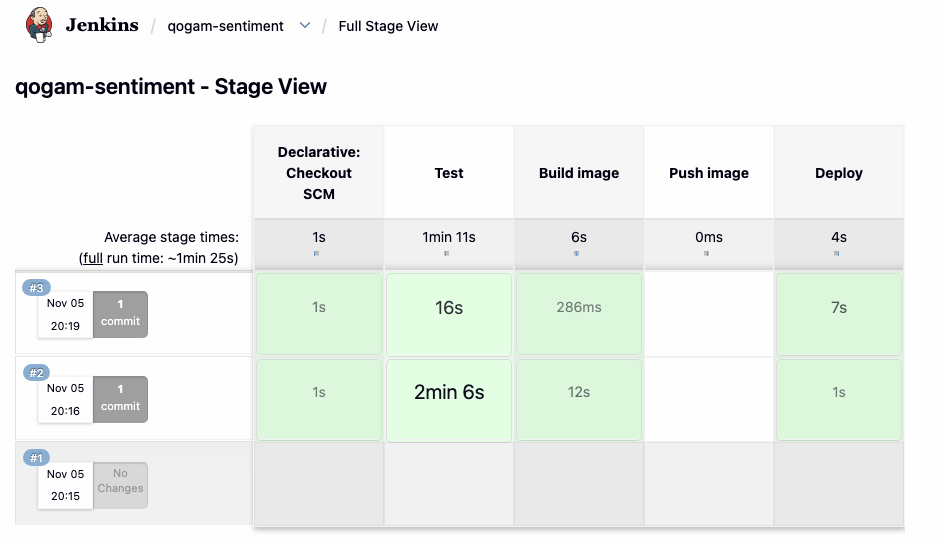
\includegraphics[height=6.2cm]{jenkins-stages.png}
\caption{Stage view of the qogam-sentiment job. Build 3 is the top row.}
\end{figure}

The deploy uses a kind cluster named \texttt{assignment5}. Kind does not see an image that exists only in Docker Desktop, so the script saves the image and imports it with \texttt{ctr}. The manifest asks for one replica and checks \texttt{/api/health}. After the import, the deployment is restarted. The tag is always \texttt{latest}, and a restart is what makes the new image the one that is running. Figure 2 is the end of the console for build 3. The new pod is up, and the build ends with SUCCESS.

\begin{figure}[H]
\centering
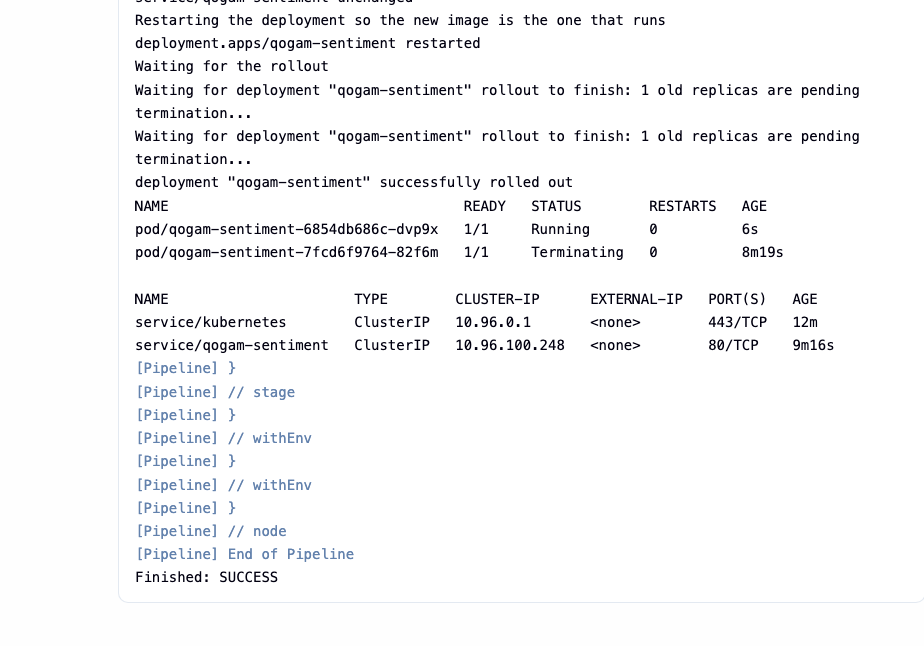
\includegraphics[height=5.0cm]{jenkins-console.png}
\caption{End of the console for build 3, including the kind rollout.}
\end{figure}

A few things took longer than the happy path. The first build failed on the timestamps option, because that option needs a plugin the image does not have. I removed the option. A normal bind mount also failed as an idea: the Docker daemon is on the Mac, and it cannot see a path that lives inside the Jenkins container. The tests are therefore streamed in with tar, while \texttt{docker build} is fine, because the client sends the files itself. The two Kubernetes files also had to be split with a document separator. Without it, only the service was created and the deployment was missing. Docker Hub is wired in the Jenkinsfile and left off, because there is no Hub account on this job.

A change on \texttt{main} is tested before an image is built, and that image can be started on the cluster without installing Python by hand. The cluster has one node. The same files are the start of a larger setup.

\end{document}
